\documentclass[8pt]{beamer}
\usetheme[block=fill]{ru}           % Use ru theme

\usepackage{common}
\usetikzlibrary{shapes.arrows}

\mode<presentation>{}


\newcommand{\chapternote}[1]{{%
  \let\thempfn\relax% Remove footnote number printing mechanism
  \footnotetext[0]{#1}% Print footnote text
}}

%% preamble
\title{Verification of Tweetnacl’s Curve25519}
% \subtitle{Coq }
\author[Beno\^{i}t Viguier MSc]{
  \normalsize Beno\^{i}t Viguier MSc \\
  {\small (\texttt{$\lambda$ x y. x@y.nl}) benoit viguier} \\
  {\small \url{https://www.viguier.nl}}\\ \medskip}

\institute[Radboud University Nijmegen]{
  Institute for Computing and Information Sciences -- Digital Security \\
  Radboud University Nijmegen}

\date[18, Mar. 2019]{
  Journée GT Méthodes Formelles pour la Sécurité\\
  March 18$^{th}$, 2019}

\setbeamertemplate{navigation symbols}{}
\begin{document}

%%%%%%%%%%%%%%%%%%%%%%%%%%%%%%%%%
%
%			SLIDE TITLE
%
%%%%%%%%%%%%%%%%%%%%%%%%%%%%%%%%%

\begin{frame}
\titlepage
\end{frame}

%%%%%%%%%%%%%%%%%%%%%%%%%%%%%%%%%
%
%     SLIDE CONTENT
%
%%%%%%%%%%%%%%%%%%%%%%%%%%%%%%%%%

\begin{frame}{Overview}
\tableofcontents
\end{frame}

\section{Prelude}

%%%%%%%%%%%%%%%%%%%%%%%%%%%%%%%%%
%
%     SLIDE 1
%
%%%%%%%%%%%%%%%%%%%%%%%%%%%%%%%%%

%%%%%%%%%%%%%%%%%%%%%%%%%%%%%%%%%
%
%			SLIDE 1
%
%%%%%%%%%%%%%%%%%%%%%%%%%%%%%%%%%
\begin{frame}[fragile]{Elliptic Curves 101}

  % \newcommand{\PP}{\mathcal{P}}
  % \newcommand{\KK}{\mathcal{K}}
  % \newcommand{\PK}{x}
  % \newcommand{\PKX}{Q}
  % \newcommand{\X}{{\bf x}}
  % \newcommand{\E}{\mathcal{E}}
  % \newcommand{\K}{\mathcal{K}}
  % \newcommand{\J}{\mathcal{J}}

  \newcommand{\XX}[1]{\ensuremath{{\textbf{x}}(#1)}}

  \begin{center}
  \begin{tikzpicture}
      \newcommand*{\xlen}{-4}
      \newcommand*{\ylen}{1.5}

      \coordinate (cquoops) at (\xlen, \ylen);
      \coordinate (cquosca) at (\xlen, \ylen-0.8);
      \coordinate (cquoadd) at (\xlen, \ylen-1.6);
      \coordinate (cquoxdbladd) at (\xlen, \ylen-2.4);

      \coordinate (cgroupops) at (\xlen, 3*\ylen);
      \coordinate (cgroupsca) at (\xlen, 3*\ylen-0.7);
      \coordinate (cgroupadd) at (\xlen, 3*\ylen-1.4);

      \node [anchor=west] (groupops) at (cgroupops)
      {\underline{\emph{Operations on $E: B y^2 = x^3 + A x^2 + x$}}};
      \node [anchor=west] (groupsca) at (cgroupsca)
      {$\textcolor{rured}{(1)}\,\,P \mapsto [2]P$};
      \node [anchor=west] (groupadd) at (cgroupadd)
      {$\textcolor{rured}{(2)}\,\,\big\{P,Q\big\}\mapsto P + Q$};

      \visible<8->{
      \node [anchor=west] (quoops) at (cquoops)
      {\underline{\emph{Operations on $\mathbb{K}$}}};
      \node [anchor=west] (quosca) at (cquosca)
      {$\textcolor{rured}{(1)}\,\,\XX{P} \mapsto \XX{[2]P}$};
      }
      \visible<16->{
      \node [anchor=west] (quoadd) at (cquoadd)
      {$\textcolor{rured}{(2)}\,\,\Big\{\XX{P},\XX{Q}\Big\}
      \mapsto \Big\{\XX{P+Q},\XX{P-Q}\Big\}$};
      }

      \visible<17->{
      \node [anchor=west] (cquoxdbladd) at (cquoxdbladd)
      {$\implies\,\,\Big\{\XX{P},\XX{Q},\XX{P-Q}\Big\}
      \mapsto \XX{P+Q}$};
      }

      \newcommand*{\aaa}{-6}
      \newcommand*{\bbb}{7}

      \newcommand*{\px}{-1.85}
      \newcommand*{\py}{3.4305}
      \newcommand*{\dfdxp}{4.2675}
      \newcommand*{\dfdyp}{-2*\py}

      \newcommand*{\pxd}{4.0868}
      \newcommand*{\pyd}{7.4716}

      \newcommand*{\qx}{0.9}
      \newcommand*{\qy}{1.5261}

      \newcommand*{\pqx}{1.42956}
      \newcommand*{\pqy}{-1.15937}

      \newcommand*{\qpx}{4.19886}
      \newcommand*{\qpy}{7.4716}

      \begin{axis}
      [
          axis x line = center,
          axis line style = thick,
          xlabel = $\mathbb{K}$,
          axis y line = none,
          ticks = none,
          xmin=-4,
          xmax=8,
          ymin=-9,
          ymax=9,
          samples=200,
          domain=-2.9005:5,
          smooth
      ]
          \addplot [rured,ultra thick] {sqrt(x^3+\aaa*x+\bbb)};
          \addplot [rured,ultra thick] {-sqrt(x^3+\aaa*x+\bbb)};

          \only<2-8>{
          \addplot [msblue,ultra thick,mark=*] coordinates {(\px,sqrt(\px^3+\aaa*\px+\bbb)};
          }

          \only<3-8>{
          \addplot [msblue,ultra thick,mark=*] coordinates {(\px,-sqrt(\px^3+\aaa*\px+\bbb)};
          }

          \only<4>{
          \draw [thick,<-,dashed] ([yshift=0.8mm]axis cs:\px,0) -- (axis cs:\px,\py);
          \draw [thick,<-,dashed] ([yshift=-0.8mm]axis cs:\px,0) -- (axis cs:\px,-\py);
          }

          \only<4->{
          \addplot [msgreen,ultra thick,mark=*] coordinates {(\px,0)};
          }

          \only<5-6>{
          \addplot [thick,dashed] {\py - (\dfdxp / \dfdyp) * ( x - \px )};
          \addplot [msyellow,ultra thick,mark=*] coordinates {(\pxd,sqrt(\pxd^3+\aaa*\pxd+\bbb)};
          }

          \only<6>{
          \draw [thick,<-,dashed] ([yshift=0.8mm]axis cs:\pxd,0) -- (axis cs:\pxd,\pyd);
          }

          \only<6-8>{
          \addplot [orange,ultra thick,mark=*] coordinates {(\pxd,0)};
          }

          \only<7>{
          \addplot [thick,dashed] {-\py - (\dfdxp / -\dfdyp) * ( x - \px )};
          \addplot [msyellow,ultra thick,mark=*] coordinates {(\pxd,-sqrt(\pxd^3+\aaa*\pxd+\bbb)};
          \draw [thick,<-,dashed] ([yshift=-0.8mm]axis cs:\pxd,0) -- (axis cs:\pxd,-\pyd);
          }

          \only<9->{
          \addplot [msgreen,ultra thick,mark=*] coordinates {(\qx,0)};
          }

          \only<10->{
          \addplot [msblue,ultra thick,mark=*] coordinates {(\px,sqrt(\px^3+\aaa*\px+\bbb)};
          \addplot [msblue,ultra thick,mark=*] coordinates {(\px,-sqrt(\px^3+\aaa*\px+\bbb)};
          \addplot [msblue,ultra thick,mark=*] coordinates {(\qx,sqrt(\qx^3+\aaa*\qx+\bbb)};
          \addplot [msblue,ultra thick,mark=*] coordinates {(\qx,-sqrt(\qx^3+\aaa*\qx+\bbb)};
          }

          \only<11>{
          \addplot [thick,dashed] { (\py - \qy) / (\px - \qx)*(x - \qx) + \qy};
          }
          \only<12>{
          \addplot [thick,dashed] { (-\py + \qy) / (\px - \qx)*(x - \qx) - \qy};
          }
          \only<13>{
          \addplot [thick,dashed] { (-\py - \qy) / (\px - \qx)*(x - \qx) + \qy};
          }
          \only<14>{
          \addplot [thick,dashed] { (\py + \qy) / (\px - \qx)*(x - \qx) - \qy};
          }

          \only<11->{
          \addplot [msyellow,ultra thick,mark=*] coordinates {(\pqx,sqrt(\pqx^3+\aaa*\pqx+\bbb)};
          }
          \only<12->{
          \addplot [msyellow,ultra thick,mark=*] coordinates {(\pqx,-sqrt(\pqx^3+\aaa*\pqx+\bbb)};
          }
          \only<13->{
          \addplot [msyellow,ultra thick,mark=*] coordinates {(\qpx,sqrt(\qpx^3+\aaa*\qpx+\bbb)};
          }
          \only<14->{
          \addplot [msyellow,ultra thick,mark=*] coordinates {(\qpx,-sqrt(\qpx^3+\aaa*\qpx+\bbb)};
          }

          \only<15>{
          \draw [thick,<-,dashed] ([yshift=0.8mm]axis cs:\pqx,0) -- (axis cs:\pqx,-\pqy);
          \draw [thick,<-,dashed] ([yshift=-0.8mm]axis cs:\pqx,0) -- (axis cs:\pqx,\pqy);
          \draw [thick,<-,dashed] ([yshift=-0.8mm]axis cs:\qpx,0) -- (axis cs:\qpx,-\qpy);
          \draw [thick,<-,dashed] ([yshift=0.8mm]axis cs:\qpx,0) -- (axis cs:\qpx,\qpy);
          }

          \only<15->{
          \addplot [orange,ultra thick,mark=*] coordinates {(\pqx,0)};
          \addplot [orange,ultra thick,mark=*] coordinates {(\qpx,0)};
          }
      \end{axis}
  \end{tikzpicture}
  \end{center}
\end{frame}


%%%%%%%%%%%%%%%%%%%%%%%%%%%%%%%%%
%
%     SLIDE 2
%
%%%%%%%%%%%%%%%%%%%%%%%%%%%%%%%%%

\begin{frame}[fragile]{Diffie-Hellman with Elliptic Curves}

  \begin{center}
  \begin{tikzpicture}
      \node[draw=none,align=center] (public) at (0,1) {Public parameter: point $P$, curve $E$ over $\mathbb{F}_p$};

      % Alice
      \node[draw] (Alice) at (-2,0) {Alice};
      \draw[->,thick,>=stealth] (Alice) -- ++(0, -4.5);

      % Calculations of Alice
      \node[draw=none,anchor=east] (asecret) at ($(Alice) + (0,-1)$) {$random\ a \in \mathbb{F}_p$};
      \node[draw=none,anchor=east] (Apublic) at ($(Alice) + (0,-2)$) {$A = [a]P$};
      \node[draw=none,anchor=east] (akey) at ($(Alice) + (0,-4)$) {$K = [a]B = [a*b]P$};

      % Bob
      \node[draw] (Bob) at (2,0) {Bob};
      \draw[->,thick,>=stealth] (Bob) -- ++(0, -4.5);

      % Calculations of Bob
      \node[draw=none,fill=none,anchor=west] (bsecret) at ($(Bob) + (0,-1)$) {$random\ b \in \mathbb{F}_p$};
      \node[draw=none,fill=none,anchor=west] (Bpublic) at ($(Bob) + (0,-2)$) {$B = [b]P$};
      \node[draw=none,fill=none,anchor=west] (bkey) at ($(Bob) + (0,-4)$) {$K = [b]A = [a*b]P$};

      % Messages
      \draw[->,thick,>=stealth] ($(Alice)+(0,-2)$) -- ($(Bob)+(0,-2.5)$) node [pos=0.5,above,font=\footnotesize] {A};
      \draw[->,thick,>=stealth] ($(Bob)+(0,-3)$) -- ($(Alice)+(0,-3.5)$) node [pos=0.5,above,font=\footnotesize] {B};
    \end{tikzpicture}
  \end{center}

\end{frame}


%%%%%%%%%%%%%%%%%%%%%%%%%%%%%%%%%
%
%     SLIDE 3
%
%%%%%%%%%%%%%%%%%%%%%%%%%%%%%%%%%
\section{Formalization of Elliptic Curves}

\begin{frame}[fragile]{Formal definition of a point}
\begin{center}
\begin{lstlisting}[language=Coq, basicstyle=\normalsize]
Inductive point (\K: Type) : Type :=
  (* A point is either at Infinity  *)
  | EC_Inf : point \K
  (* or (x,y) *)
  | EC_In  : \K -> \K -> point \K.

Notation "\infty" := (@EC_Inf _).
Notation "(| x , y |)" := (@EC_In _ x y).



(* Get the x coordinate of p or 0 *)
Definition point_x0 (p : point \K) :=
  if p is (|x, _ |) then x else 0.

Notation "p.x" := (point_x0 p).
\end{lstlisting}
\end{center}
\chapternote{A Formal Library for Elliptic Curves in the Coq Proof Assistant --
Evmorfia-Iro Bartzia, Pierre-Yves Strub
\url{https://hal.inria.fr/hal-01102288}}
\end{frame}




\begin{frame}[fragile]{Formal definition of a curve}
\begin{center}
\begin{lstlisting}[language=Coq, basicstyle=\normalsize]
(* Definition of a curve in its Montgomery form *)
(* B y = x^3 + A x^2 + x *)
Record mcuType := {
  A: \K;
  B: \K;
  _ : B != 0;
  _ : A^2 != 4
}


(* is a point p on the curve? *)
Definition oncurve (p: point \K) : bool :=
  match p with
  | \infty => true
  | (| x , y |) => B * y^2 == x^3 + A * x^2 + x
  end.

(* We define a point on a curve as a point
   and the proof that it is on the curve *)
Inductive mc : Type :=
  MC p of oncurve p.
\end{lstlisting}
\end{center}
\end{frame}
% \begin{frame}[fragile]{Formal definition of the operations over a curve}
% \begin{center}
% \begin{lstlisting}[language=Coq]
% Definition neg (p: point \K) :=
%   if p is (| x, y |) then (| x, - y |) else \infty.
%
%
% Definition add (p1 p2: point \K) :=
%     let p1 := if oncurve p1 then p1 else \infty in    (* Making sure p1 and p2 are on the curve *)
%     let p2 := if oncurve p2 then p2 else \infty in
%
%     match p1 , p2 with
%     | \infty, _ => p2                                 (* If one point is infinity *)
%     | _, \infty => p1                                 (* If one point is infinity *)
%
%     | (| x1, y1 |), (| x2, y2 |) =>
%       if x1 == x2 then
%         if (y1 == y2) && (y1 != 0) then                             (* If p1 = p2 *)
%           let s := (3 * x1^2 + 2 * A * x1 + 1) / (2 * B * y1) in
%           let xs := s^2 * B - A - 2*x1 in
%             (| xs, -s * (xs - x1) - y1 |)
%         else
%           \infty
%       else                                                          (* If p1 <> p2 *)
%         let s := (y2 - y1) / (x2 - x1) in
%         let xs := s^2 * B - A - x1 - x2 in
%          (| xs, -s * (xs - x1) - y1|)
%     end
%
%
% Notation "- x" := (neg x).
% Notation "x + y" := (add x y).
% Notation "x - y" := (x + (- y)).
% \end{lstlisting}
% \end{center}
% \end{frame}

%%%%%%%%%%%%%%%%%%%%%%%%%%%%%%%%%
%
%     SLIDE 4
%
%%%%%%%%%%%%%%%%%%%%%%%%%%%%%%%%%

\begin{frame}[fragile]{Montgomery ladder}
\begin{center}
\begin{lstlisting}[language=Coq]
Definition cswap (c : \N) (a b : \K) :=
  if c == 1 then (b, a) else (a, b).

Fixpoint opt_montgomery_rec (n m : \N) (x a b c d : \K) : \K :=
  if m is m.+1 then
    let (a, b) := cswap (bitn n m) a b in
    let (c, d) := cswap (bitn n m) c d in
    let e := a + c in
    let a := a - c in
    let c := b + d in
    let b := b - d in
    let d := e^2 in
    let f := a^2 in
    let a := c * a in
    let c := b * e in
    let e := a + c in
    let a := a - c in
    let b := a^2 in
    let c := d - f in
    let a := c * ((A - 2) / 4) in
    let a := a + d in
    let c := c * a in
    let a := d * f in
    let d := b * x in
    let b := e^2 in
    let (a, b) := cswap (bitn n m) a b in
    let (c, d) := cswap (bitn n m) c d in
    opt_montgomery_rec n m x a b c d
  else
    a / c.

Definition opt_montgomery (n m : \N) (x : \K) : \K :=
  opt_montgomery_rec n m x 1 x 0 1.
\end{lstlisting}
\end{center}
\end{frame}

%%%%%%%%%%%%%%%%%%%%%%%%%%%%%%%%%
%
%     SLIDE 5
%
%%%%%%%%%%%%%%%%%%%%%%%%%%%%%%%%%

\begin{frame}[fragile]{Correctness of the montgomery ladder}
\begin{center}
\begin{lstlisting}[language=Coq, basicstyle=\large]







Lemma opt_montgomery_ok :
  forall (n m: \N) (xp : \K) (P : mc M),
  n << 2^m
  -> xp != 0

  -> P.x = xp
    (* if xp is the x coordinate of P *)

  -> opt_montgomery n m xp = ([n]P).x
    (* opt_montgomery n m xp is the x coordinate of [n]P *)
  .
\end{lstlisting}
\end{center}
\end{frame}

%%%%%%%%%%%%%%%%%%%%%%%%%%%%%%%%%
%
%     SLIDE 6
%
%%%%%%%%%%%%%%%%%%%%%%%%%%%%%%%%%

\begin{frame}[fragile]{Correctness of the Curve25519 ladder}
\begin{center}
\begin{lstlisting}[language=Coq, basicstyle=\large]
(* \K = \GF *)
(* A = 486662   *)
(* B = 1        *)
(* Curve25519 : y^2 = x^3 + 486662 * x^2 + x *)

Definition curve25519_ladder n x = opt_montgomery n 255 x.

Lemma curve25519_ladder_ok :
  forall (n: \N) (xp : \GF) (P : mc Curve25519),
  n << 2^255
  -> xp != 0

  -> P.x = xp
    (* if xp is the x coordinate of P *)

  -> curve25519_ladder n xp = ([n]P).x
    (* curve25519_ladder n xp is the x coordinate of [n]P *)
  .
\end{lstlisting}
\end{center}
\end{frame}

\section{A quick overview of TweetNaCl}

%%%%%%%%%%%%%%%%%%%%%%%%%%%%%%%%%
%
%			SLIDE 7
%
%%%%%%%%%%%%%%%%%%%%%%%%%%%%%%%%%
\begin{frame}[fragile]{crypto\_scalarmult}
  \vspace{-0.5cm}
  \begin{center}
\begin{lstlisting}[language=Ctweetnacl]
int crypto_scalarmult(u8 *q,const u8 *n,const u8 *p)
{
  u8 z[32]; i64 r; int i; gf x,a,b,c,d,e,f;
  FOR(i,31) z[i]=n[i];
  z[31]=(n[31]&127)|64; z[0]&=248;                #   Clamping of n
  unpack25519(x,p);
  FOR(i,16) { b[i]=x[i]; d[i]=a[i]=c[i]=0; }
  a[0]=d[0]=1;
  for(i=254;i>=0;--i) {
    r=(z[i>>3]>>(i&7))&1;                         #   i^th bit of n
    sel25519(a,b,r);
    sel25519(c,d,r);
    A(e,a,c);                                     #
    Z(a,a,c);                                     #
    A(c,b,d);                                     #
    Z(b,b,d);                                     #
    S(d,e);                                       #
    S(f,a);                                       #
    M(a,c,a);                                     #  Montgomery Ladder
    M(c,b,e);                                     #
    A(e,a,c);                                     #
    Z(a,a,c);                                     #
    S(b,a);                                       #
    Z(c,d,f);                                     #
    M(a,c,_121665);                               #
    A(a,a,d);                                     #
    M(c,c,a);                                     #
    M(a,d,f);                                     #
    M(d,b,x);                                     #
    S(b,e);                                       #
    sel25519(a,b,r);
    sel25519(c,d,r);
  }
  inv25519(c,c); M(a,a,c);                        #   a / c
  pack25519(q,a);
  return 0;
}
\end{lstlisting}
\end{center}
  % \chapternote{\url{https://tweetnacl.cr.yp.to}}

\end{frame}

%%%%%%%%%%%%%%%%%%%%%%%%%%%%%%%%%
%
%     SLIDE 8
%
%%%%%%%%%%%%%%%%%%%%%%%%%%%%%%%%%
\begin{frame}[fragile]{Number representation}
  \begin{center}

  256 bits integers does not fit into a 64 bits containers...

  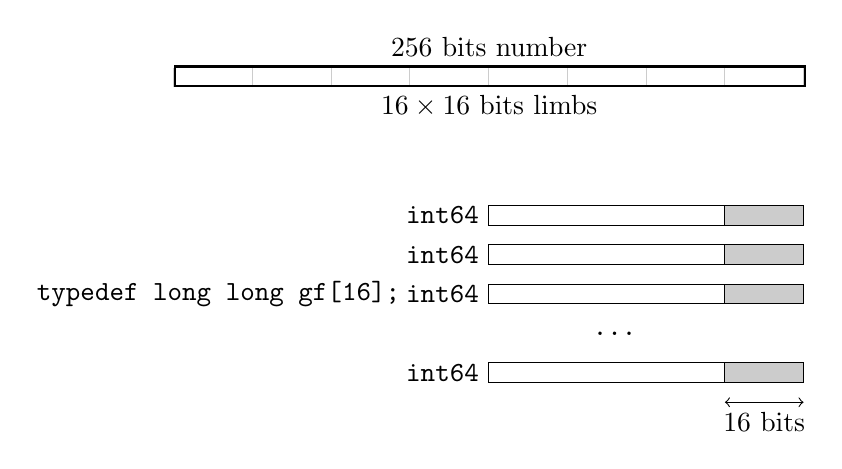
\begin{tikzpicture}[textstyle/.style={black, anchor= south west, align=center}]


  \foreach \x in {0,1,...,8} {
    \draw [black!20] (\x,0) -- (\x,0.25);
  };

  \draw (0,0.25) node[textstyle, minimum width=8cm, minimum height=0.5cm] {$256$ bits number};
  \draw (0,0) node[textstyle, draw=black, thick, minimum width=8cm, minimum height=0.25cm] {};

  \draw (0,-0.5) node[textstyle, minimum width=8cm] {$16 \times 16$ bits limbs};

  \def\yshift{-1.5}
  \def\xshift{4}

  \foreach \y in {0,-0.5,-1,-2} {
    \draw (\xshift+0,\yshift+\y) -- (\xshift+4,\yshift+\y) -- (\xshift+4,\yshift-0.25+\y) -- (\xshift+0,\yshift-0.25+\y) -- cycle;
    \draw [fill=black!20] (\xshift+3,\yshift+\y) -- (\xshift+4,\yshift+\y) -- (\xshift+4,\yshift-0.25+\y) -- (\xshift+3,\yshift-0.25+\y) -- cycle;
    \draw (\xshift,\yshift-0.125+\y) node[anchor= east, align=center] {\texttt{int64}};
  }
  \draw (\xshift+2,\yshift-0.125-1.5) node[anchor= east, align=center] {\texttt{...}};

  \draw (3,\yshift-1.125) node[anchor= east, align=center] {\texttt{typedef long long gf[16];}};

  \def\yshift{-4}
  \draw [<->] (\xshift+3,\yshift) -- (\xshift+4,\yshift);
  \draw (\xshift+3.5,\yshift) node[textstyle, anchor=north] {$16$ bits};
  \end{tikzpicture}
  \end{center}
\end{frame}


%%%%%%%%%%%%%%%%%%%%%%%%%%%%%%%%%
%
%     SLIDE 9
%
%%%%%%%%%%%%%%%%%%%%%%%%%%%%%%%%%
\begin{frame}[fragile]{Basic Operations}
  \begin{center}

\begin{lstlisting}[language=cnacl]
#define FOR(i,n) for (i = 0;i < n;++i)
#define sv static void
typedef long long i64;
typedef i64 gf[16];


sv A(gf o,const gf a,const gf b)    # Addition
{
  int i;
  FOR(i,16) o[i]=a[i]+b[i];         # carrying is done separately
}


sv Z(gf o,const gf a,const gf b)    # Zubstraction
{
  int i;
  FOR(i,16) o[i]=a[i]-b[i];         # carrying is done separately
}


sv M(gf o,const gf a,const gf b)    # Multiplication (school book)
{
  i64 i,j,t[31];
  FOR(i,31) t[i]=0;
  FOR(i,16) FOR(j,16) t[i+j] = a[i]*b[j];
  FOR(i,15) t[i]+=38*t[i+16];
  FOR(i,16) o[i]=t[i];
  car25519(o);                      # carrying
  car25519(o);                      # carrying
}
\end{lstlisting}

  \end{center}
\end{frame}

\section{From C to Coq}

%%%%%%%%%%%%%%%%%%%%%%%%%%%%%%%%%
%
%     SLIDE 10
%
%%%%%%%%%%%%%%%%%%%%%%%%%%%%%%%%%

\begin{frame}[fragile]{Proving with VST}
  \begin{center}

  \begin{tikzpicture}[textstyle/.style={black, anchor= south west, align=center}]
      \draw (2.75,0) node[textstyle, anchor=west, draw=none, fill=doc@lstbackground, thick, minimum width=5.5cm,minimum height=5cm] {};
      \node[inner sep=0pt] (russell) at (5.5,1.5) {
\includegraphics[width=.1\textwidth]{coq_logo.png}};
      \node[inner sep=0pt] (russell) at (5.5,-1.5) {
\includegraphics[width=.15\textwidth]{chain.png}};
      \draw (-1,0) node[textstyle, anchor=east, draw=black, thick, minimum width=1cm,minimum height=2cm] {code.c};
      \draw (0.75,-0.5) node[textstyle, anchor=south] {\texttt{clightgen code.c}};
      \draw (4,0) node[textstyle, anchor=east, draw=black, thick, minimum width=1cm,minimum height=2cm] {code.v};
      \draw (8,0) node[textstyle, anchor=east, draw=black, thick, minimum width=1cm,minimum height=2cm] {proofs.v};
      \node[anchor=west,single arrow,draw=red!80!black,fill=red!80!black,minimum width=0.5cm,minimum height=3.25cm] at (-0.75,0) {};
      \node[anchor=west,double arrow,draw=green!60!black,fill=green!60!black,minimum width=0.5cm,minimum height=2.25cm] at (4.25,0) {};
      % \node[anchor=west,double arrow,draw=green!60!black,fill=green!60!black,minimum width=0.5cm,minimum height=2cm] at (3,0) {};
  \end{tikzpicture}

  \end{center}
\end{frame}


%%%%%%%%%%%%%%%%%%%%%%%%%%%%%%%%%
%
%     SLIDE 11
%
%%%%%%%%%%%%%%%%%%%%%%%%%%%%%%%%%

\begin{frame}[fragile]{Specification: ZofList}
  \begin{center}
\begin{lstlisting}[language=Coq, basicstyle=\normalsize]
Variable n: \Z.
Hypothesis Hn: n > 0.


(*
  in C we have gf[16] here we consider a list of integers (list \Z)
  of length 16 in this case.

  ZofList convert a list \Z into it's \Z value
  assume a radix: 2^n
*)
Fixpoint ZofList (a : list \Z) : \Z :=
  match a with
  | [] => 0
  | h :: q => h + 2^n * ZofList q
  end.

Notation "\Z.of_list A" := (ZofList A).
\end{lstlisting}
  \end{center}
\end{frame}


%%%%%%%%%%%%%%%%%%%%%%%%%%%%%%%%%
%
%     SLIDE 12
%
%%%%%%%%%%%%%%%%%%%%%%%%%%%%%%%%%

\begin{frame}[fragile]{Specification: Addition}
  \begin{center}
\begin{lstlisting}[language=Coq]
Fixpoint A (a b : list \Z) : list \Z :=
  match a,b with
  | [], q => q
  | q,[] => q
  | h1::q1,h2::q2 => (Z.add h1 h2) :: A q1 q2
  end.
Notation "a \boxplus b" := (A a b) (at level 60).


Corollary A_correct:
  forall (a b: list \Z),
    \Z.of_list (a \boxplus b) = (\Z.of_list a) + (\Z.of_list b).
Qed.


Lemma A_bound_len:
  forall (m1 n1 m2 n2: \Z) (a b: list \Z),
    length a = length b ->
    Forall (fun x => m1 << x << n1) a ->
    Forall (fun x => m2 << x << n2) b ->
      Forall (fun x => m1 + m2 < x < n1 + n2) (a \boxplus b).
Qed.

Lemma A_length_16:
  forall (a b: list \Z),
  length a = 16 ->
  length b = 16 ->
    length (a \boxplus b) = 16.
Qed.
\end{lstlisting}

  \end{center}
\end{frame}





\begin{frame}[fragile]{Verification: Addition (with VST)}
\begin{center}
\begin{tikzpicture}
\draw (0,0) node[below left] {
\begin{lstlisting}[language=CoqVST]
Definition A_spec :=
DECLARE _A
WITH
  v_o: val, v_a: val, v_b: val,
  sh : share,
  o : list val,
  a : list Z, amin : Z, amax : Z,
  b : list Z, bmin : Z, bmax : Z,

(*------------------------------------------*)
PRE [ _o OF (tptr tlg), _a OF (tptr tlg), _b OF (tptr tlg) ]
    PROP  (writable_share sh;
          (* For soundness *)                         (* For bounds propagation *)
           Forall (fun x => -2^62 < x < 2^62) a;          Forall (fun x => amin < x < amax) a;
           Forall (fun x => -2^62 < x < 2^62) b;          Forall (fun x => bmin < x < bmax) b;

           Zlength a = 16; Zlength b = 16; Zlength o = 16)
    LOCAL (temp _a v_a; temp _b v_b; temp _o v_o)
    SEP   (sh [{ v_o }] <<(lg16)-- o;
           sh [{ v_a }] <<(lg16)-- mVI64 a;
           sh [{ v_b }] <<(lg16)-- mVI64 b)

  (*------------------------------------------*)
  POST [ tvoid ]
      PROP ( (* Bounds propagation *)
            Forall (fun x => amin + bmin < x < amax + bmax) (A a b)
            Zlength (A a b) = 16;
           )
      LOCAL()
      SEP (sh [{ v_o }] <<(lg16)-- mVI64 (A a b);
           sh [{ v_a }] <<(lg16)-- mVI64 a;
           sh [{ v_b }] <<(lg16)-- mVI64 b).
\end{lstlisting}
};
\draw (1.5,0) node[below left] {
\begin{lstlisting}[language=cnacl]
sv A(gf o,const gf a,const gf b)
{
  int i;
  FOR(i,16) o[i]=a[i]+b[i];
}
\end{lstlisting}
};
\draw[black] (1.5,0) -- (1.5,-1.35) -- (-2.35,-1.35) -- (-2.35,0) -- cycle;
\end{tikzpicture}
\end{center}
\end{frame}


\begin{frame}[fragile]{Using VST}
\begin{lstlisting}[language=CoqVST]
Definition crypto_scalarmult_spec :=
DECLARE _crypto_scalarmult_curve25519_tweet
WITH
  v_q: val, v_n: val, v_p: val, c121665:val,
  sh : share,
  q : list val, n : list Z, p : list Z

(*------------------------------------------*)
PRE [ _q OF (tptr tuchar), _n OF (tptr tuchar), _p OF (tptr tuchar) ]
    PROP (writable_share sh;
          Forall (fun x => 0 <= x < 2^8) p;
          Forall (fun x => 0 <= x < 2^8) n;
          Zlength q = 32; Zlength n = 32; Zlength p = 32 )
    LOCAL(temp _q v_q; temp _n v_n; temp _p v_p; gvar __121665 c121665 )
    SEP  (sh [{ v_q }] <<(uch32)-- q;
          sh [{ v_n }] <<(uch32)-- mVI n;
          sh [{ v_p }] <<(uch32)-- mVI p;
          Ews [{ c121665 }] <<(lg16)-- mVI64 c_121665)

(*------------------------------------------*)
POST [ tint ]
    PROP (Forall (fun x => 0 <= x < 2^8) (Crypto_Scalarmult n p);
          Zlength (Crypto_Scalarmult n p) = 32)
    LOCAL(temp ret_temp (Vint Int.zero))
    SEP  (sh [{ v_q }] <<(uch32)-- mVI (Crypto_Scalarmult n p);
          sh [{ v_n }] <<(uch32)-- mVI n;
          sh [{ v_p }] <<(uch32)-- mVI p;
          Ews [{ c121665 }] <<(lg16)-- mVI64 c_121665
\end{lstlisting}
\end{frame}

\section{Crypto\_Scalarmult n P.x = ([n]P).x ?}

\begin{frame}[fragile]{Generic Operations}
\begin{center}

\begin{lstlisting}[language=Coq]
Class Ops (T T': Type) (Mod: T -> T):=
{
  A:   T -> T -> T;                 (* Addition       over T *)
  M:   T -> T -> T;                 (* Multiplication over T *)
  Zub: T -> T -> T;                 (* Substraction   over T *)
  Sq:  T -> T;                       (* Squaring       over T *)
  C_0: T;                             (* Constant 0       in T *)
  C_1: T;                             (* Constant 1       in T *)
  C_121665: T;                        (* Constant 121665  in T *)
  Sel25519: \Z -> T -> T -> T;      (* Select the 2^nd or 3^rd argument depending of Z *)
  Getbit:   \Z -> T' -> \Z;           (* Return the i^th bit of T' *)

  (* Mod conservation *)
  Mod_ZSel25519_eq : forall b p q,  Mod (Sel25519 b p q) = Sel25519 b (Mod p) (Mod q);
  Mod_ZA_eq :        forall p q,    Mod (A p q)          = Mod (A (Mod p) (Mod q));
  Mod_ZM_eq :        forall p q,    Mod (M p q)          = Mod (M (Mod p) (Mod q));
  Mod_ZZub_eq :      forall p q,    Mod (Zub p q)        = Mod (Zub (Mod p) (Mod q));
  Mod_ZSq_eq :       forall p,      Mod (Sq p)           = Mod (Sq (Mod p));

  Mod_red :          forall p,      Mod (Mod p)          = (Mod p)
}.
\end{lstlisting}
\end{center}
\end{frame}

\begin{frame}[fragile]{Generic Montgomery Ladder}
\begin{center}
\begin{lstlisting}[language=Coq]
Context {T : Type}.
Context {T' : Type}.
Context {Mod : T -> T}.
Context {O : Ops T T' Mod}.

Fixpoint montgomery_rec (m : \N) (z : T') (a b c d e f x : T) : (T * T * T * T * T * T) :=
  match m with
  | 0 => (a,b,c,d,e,f)
  | S n =>
      let r := Getbit (\Z.of_nat n) z in
      let (a, b) := (Sel25519 r a b, Sel25519 r b a) in
      let (c, d) := (Sel25519 r c d, Sel25519 r d c) in
      let e := A a c in
      let a := Zub a c in
      let c := A b d in
      let b := Zub b d in
      let d := Sq e in
      let f := Sq a in
      let a := M c a in
      let c := M b e in
      let e := A a c in
      let a := Zub a c in
      let b := Sq a in
      let c := Zub d f in
      let a := M c C_121665 in
      let a := A a d in
      let c := M c a in
      let a := M d f in
      let d := M b x in
      let b := Sq e in
      let (a, b) := (Sel25519 r a b, Sel25519 r b a) in
      let (c, d) := (Sel25519 r c d, Sel25519 r d c) in
      montgomery_rec n z a b c d e f x
    end.
\end{lstlisting}
\end{center}
\end{frame}

\begin{frame}[fragile]{Operations Equivalence}
\begin{center}

\begin{lstlisting}[language=Coq]
Class Ops_Mod_P {T T' U:Type}
                {Mod:U -> U} {ModT:T -> T}
                `(Ops T T' ModT) `(Ops U U Mod)  :=
{
P:  T  -> U;    (* Projection from T  to U *)
P': T' -> U;    (* Projection from T' to U *)

A_eq:        forall a b, Mod (P (A a b))   = Mod (A (P a) (P b));
M_eq:        forall a b, Mod (P (M a b))   = Mod (M (P a) (P b));
Zub_eq:      forall a b, Mod (P (Zub a b)) = Mod (Zub (P a) (P b));
Sq_eq:       forall a,   Mod (P (Sq a))    = Mod (Sq (P a));

C_121665_eq: P C_121665 = C_121665;
C_0_eq:      P C_0 = C_0;
C_1_eq:      P C_1 = C_1;

Sel25519_eq: forall b p q,  Mod (P (Sel25519 b p q)) = Mod (Sel25519 b (P p) (P q));
Getbit_eq:   forall i p,    Getbit i p = Getbit i (P' p);
}.
\end{lstlisting}
\end{center}
\end{frame}


\begin{frame}[fragile]{Generic Montgomery Equivalence}
\begin{center}

\begin{lstlisting}[language=Coq]
Context {T:    Type}.
Context {T':   Type}.
Context {U:    Type}.
Context {ModT: T -> T}.
Context {Mod:  U -> U}.
Context {TO:   Ops T T' ModT}.
Context {UO:   Ops U U  Mod}.
Context {UTO: @Ops_Mod_P T T' U Mod ModT TO UO}.


(* montgomery_rec over T is equivalent to montgomery_rec over U *)
Corollary montgomery_rec_eq_a: forall (n:\N) (z:T') (a b c d e f x: T),
  0 <= m ->
  Mod (P (get_a (montgomery_rec n z a b c d e f x))) =                              (* over T *)
  Mod (get_a (montgomery_rec n (P' z) (P a) (P b) (P c) (P d) (P e) (P f) (P x))).  (* over U *)
Qed.

Corollary montgomery_rec_eq_c: forall (n:\N) (z:T') (a b c d e f x: T),
  0 <= m ->
  Mod (P (get_c (montgomery_rec n z a b c d e f x))) =                              (* over T *)
  Mod (get_c (montgomery_rec n (P' z) (P a) (P b) (P c) (P d) (P e) (P f) (P x))).  (* over U *)
Qed.
\end{lstlisting}
\end{center}
\end{frame}


\begin{frame}[fragile]{Instanciating}
\vspace{-0.5cm}
\begin{center}
\begin{lstlisting}[language=Coq]
Definition modP (x: \Z) := x mod 2^255-19.

(* Operations over \Z *)
Instance Z_Ops :      Ops \Z \Z modP := {}.

(* Operations over \GF *)
Instance Z25519_Ops : Ops \GF \N id := {}.

(* Equivalence between \Z (with modP) and \Z *)
Instance Zmod_Z_Eq :   @Ops_Mod_P Z Z Z modP modP Z_Ops Z_Ops :=
{ P := modP; P' := id }.

(* Equivalence between \Z (with modP) and \GF *)
Instance Z25519_Z_Eq : @Ops_Mod_P Zmodp.type nat Z modP id Z25519_Ops Z_Ops :=
{ P := val; P' := \Z.of_nat }.

Inductive List16 (T:Type) := Len (l:list T): Zlength l = 16 -> List16 T.
Inductive List32B :=         L32B (l:list \Z): Forall (fun x => 0 <= x << 2^8) l -> List32B.

(* Operations over List16,List32 *)
Instance List16_Ops : Ops (@List16 \Z) List32B id := {}.

(* Equivalence between List16,List32 and \Z *)
Instance List16_Z_Eq : @Ops_Mod_P (@List16 \Z) (List32B) Z Mod id List16_Ops Z_Ops :=
{  P l := (ZofList 16 (List16_to_List l));       P' l := (ZofList 8 (List32_to_List l));  }.

(* Operations over list of \Z *)
Instance List_Z_Ops : Ops (list \Z) (list \Z) id := {}.

(* Equivalence between List16,List32 and list of \Z *)
Instance List16_List_Z_Eq : @Ops_Mod_P (List16 \Z) (List32B) (list \Z) id id List16_Ops List_Z_Ops :=
{  P := List16_to_List;         P' := List32_to_List      }.
\end{lstlisting}
\end{center}
\end{frame}


\begin{frame}[fragile]{Full Equivalence}
\vspace{-0.2cm}
\begin{center}
\begin{tikzpicture}

\draw[draw=none,fill=doc@lstbackground] (-8,1) -- (3,1) -- (3,-7.5) -- (-8,-7.5) -- cycle;
\draw (-8,-7.5) node[inner sep=0pt, above right] {
\includegraphics[width=.1\textwidth]{coq_logo.png}};

\draw (0,0) node[above,draw, minimum width=4cm, minimum height=0.65cm] (GF) {\coqes{Ops \GF \N id}};
\draw (0,-1.5) node[above,draw, minimum width=4cm, minimum height=0.65cm] (Zmod) {\coqes{Ops \Z(with modP) \Z(with modP) modP}};
\draw (0,-3) node[above,draw, minimum width=4cm, minimum height=0.65cm] (Z) {\coqes{Ops \Z \Z modP}};
\draw (0,-4.5) node[above,draw, minimum width=4cm, minimum height=0.65cm] (L16) {\coqes{Ops (@List16 \Z) List32B id}};
\draw (0,-6) node[above,draw, minimum width=4cm, minimum height=0.65cm] (L) {\coqes{Ops (list \Z) (list \Z) id}};

\draw[double,<->,>=stealth] (GF.south) -- (Zmod.north) node[midway, right]{\coqes{Z25519_Z_Eq}};
\draw[double,<->,>=stealth] (Zmod.south) -- (Z.north) node[midway, right]{\coqes{Zmod_Z_Eq}};
\draw[double,<->,>=stealth] (Z.south) -- (L16.north) node[midway, right]{\coqes{List16_Z_Eq}};
\draw[double,<->,>=stealth] (L16.south) -- (L.north) node[midway, right]{\coqes{List16_List_Z_Eq}};

\draw[<-] (GF.west) --++ (-1.5,0) node[left] {\coqes{curve25519_ladder n xp}}                     node[midway,above] {\scriptsize defined with};
\draw[<-] (Z.west)  --++ (-1.5,0) node[left] {\coqes{ZCrypto_Scalarmult (ZofList n) (ZofList p)}}  node[midway,above] {\scriptsize defined with};
\draw[<-] (L.west)  --++ (-1.5,0) node[left] (CSM) {\coqes{Crypto_Scalarmult n p}}                 node[midway,above] {\scriptsize defined with};

\draw (-6.25,-7.4) node[above right,draw,dashed,minimum width=3.5cm, minimum height=0.45cm] (TNACL) {\scriptsize \texttt{tweetnacl.v} (output of clightgen)};

\draw[double,<->,>=stealth] (CSM.south) -- (TNACL.north) node[midway, right]{
\includegraphics[width=.07\textwidth]{chain.png}};

\end{tikzpicture}

\end{center}
\end{frame}



\begin{frame}[fragile]{Final Theorems}
\vspace{-0.5cm}
\begin{center}

% Definition Crypto_Scalarmult n p :=
%   let N := clamp n in
%   let P := Unpack25519 p in
%   let t := montgomery_rec 255 N C_1 P C_0 C_1 C_0 C_0 P in
%   Pack25519 (Low.M (get_a t) (Inv25519 (get_c t))).
%
% Definition ZCrypto_Scalarmult n p :=
%   let N := Zclamp n in
%   let P := ZUnpack25519 p in
%   let t := montgomery_rec 255 N 1 P 0 1 0 0 P in
%   ZPack25519 (Z.mul (get_a t) (ZInv25519 (get_c t))).
%
% Lemma ZCrypto_Scalarmult_curve25519_ladder n x :
%   ZCrypto_Scalarmult n x =
%       val (curve25519_ladder (Z.to_nat (Zclamp n))
%                              (Zmodp.pi (modP (ZUnpack25519 x)))).

\begin{lstlisting}[language=Coq]
Theorem Crypto_Scalarmult_Eq :
  forall (n p:list \Z),

  Zlength n = 32 ->                               (* n is a list of 32 unsigned bytes *)
  Forall (fun x => 0 <= x /\ x << 2^8) n ->

  Zlength p = 32 ->                               (* p is a list of 32 unsigned bytes *)
  Forall (fun x => 0 <= x /\ x << 2^8) p ->

  ZofList 8 (Crypto_Scalarmult n p) =
      val (curve25519_ladder (Z.to_nat (Zclamp (ZofList 8 n)))
                             (Zmodp.pi (modP (ZUnpack25519 (ZofList 8 p))))).

 (* The operations in Crypto_Scalarmult converted to \Z yield   *)
 (* to the exact same result as the ladder over \GF       *)




Lemma curve25519_ladder_ok :
   forall (n: \N) (xp : \GF) (P : mc Curve25519),
   n << 2^255
   -> xp != 0

   -> P.x = xp
     (* if xp is the x coordinate of P *)

   -> curve25519_ladder n xp = ([n]P).x.
     (* curve25519_ladder n xp is the x coordinate of [n]P *)
\end{lstlisting}
\end{center}
\end{frame}

%
% \begin{frame}[standout]
%   \Huge What's left ?
% \end{frame}
%
% \begin{frame}[fragile]
%     \begin{itemize}
%       \item[\color{ruDarkTeal}$\blacktriangleright$] Adding some glue between this theorem and the lemma.
%       \item[\color{ruDarkTeal}$\blacktriangleright$] Twist ?.
%     \end{itemize}
% \end{frame}
%




% %%%%%%%%%%%%%%%%%%%%%%%%%%%%%%%%%
% %
% %     SLIDE 10
% %
% %%%%%%%%%%%%%%%%%%%%%%%%%%%%%%%%%
%
% \begin{frame}[fragile]{Multiplication - specification}
%   \begin{center}
% \begin{lstlisting}[language=cnacl, caption=M, label=cod:languageC101]
% sv M(gf o,const gf a,const gf b)    # Multiplication
% {
%   FOR(i,16) FOR(j,16) t[i+j] = a[i]*b[j];   # mult_1
%   FOR(i,15) t[i]+=38*t[i+16];               # mult_2
%   FOR(i,16) o[i]=t[i];                      # mult_3
%  }
% \end{lstlisting}
%
% \begin{lstlisting}[language=Coq, caption=Multiplication, label=cod:languageC102]
% Fixpoint ZscalarMult (a: \Z) (b: list \Z) : list \Z := match b with
% | [] => []
% | h :: q => a * h :: ZscalarMult a q
% end.
% Notation "A \circ B" := (ZscalarMult A B) (at level 60).
%
% Fixpoint mult_1 (a b:list \Z) : list \Z := match a, b with
% | [],_ => []
% | _,[] => []
% | ha :: qa, hb :: qb => ha * hb :: (ha \circ qb) \boxplus (mult_1 qa (hb::qb))
% end.
%
% Definition mult_2 (a:list \Z) : list \Z := a  \boxplus (38 \circ (tail 16 a)).
% (* where "tail n a" drop the n first elements of a *)
%
% Definition mult_3 (a:list \Z) : list \Z := slice 16 a.
% (* where "slice n a" keep the n first elements of a *)
%
% Definition M (a b:list \Z) : list \Z := mult_3 (mult_2 (mult_1 a b)).
% \end{lstlisting}
%
%   \end{center}
% \end{frame}
%
% %%%%%%%%%%%%%%%%%%%%%%%%%%%%%%%%%
% %
% %     SLIDE 11
% %
% %%%%%%%%%%%%%%%%%%%%%%%%%%%%%%%%%
%
% \begin{frame}[fragile]{Multiplication - correctness}
%   \begin{center}
% \begin{lstlisting}[language=Coq, caption=Multiplication | proof of correctness, label=cod:languageC111]
% Notation "A :\GF" := (A mod (2^255-19)) (at level 40).
%
% Corollary mult1_correct :
%   forall (a b: list \Z),
%     \Z.of_list mult_1 a b =  (\Z.of_list a) * (\Z.of_list b).
% Qed.
%
% Lemma mult_2_correct :
%   forall (l: list \Z),
%     (\Z.of_list mult_2 l) = (\Z.of_list l) + 38 * \Z.of_list tail 16 l.
% Qed.
%
% Lemma reduce_slice_GF:
%   forall (l: list \Z),
%     \Z.\N length l < 32 ->
%       (\Z.of_list mult_3 (mult_2 l)) :\GF = (\Z.of_list l) :\GF.
% Qed.
%
% Corollary mult_GF:
%   forall (a b: list \Z),
%     \Z.\N length a = 16 ->
%     \Z.\N length b = 16 ->
%       (\Z.of_list M a b) :\GF = (\Z.of_list a) * (\Z.of_list b) :\GF.
% Qed.
% \end{lstlisting}
%
%   \end{center}
% \end{frame}


%%%%%%%%%%%%%%%%%%%%%%%%%%%%%%%%%
%
%     SLIDE 12
%
%%%%%%%%%%%%%%%%%%%%%%%%%%%%%%%%%

% \begin{frame}[fragile]{Multiplication - base lemma}
%   \begin{center}
% \begin{lstlisting}[language=Coq, caption=Base lemma for the multiplication, label=cod:languageC121]
% Definition min_prod (min1 max1 min2 max2: \Z) : \Z :=
%   Zmin (Zmin (min1*min2) (max1*max2)) (Zmin (max1*min2) (min1*max2)).

% Definition max_prod (min1 max1 min2 max2: \Z) : \Z :=
%   Zmax (Zmax (min1*min2) (max1*max2)) (Zmax (max1*min2) (min1*max2)).

% Lemma Mult_interval_correct_min_max_lt :
%   forall a b c d x y : \Z,
%     a < x < b ->
%     c < y < d ->
%     min_prod a b c d < x * y < max_prod a b c d.
% Qed.
% \end{lstlisting}

%   \end{center}
% \end{frame}

% %%%%%%%%%%%%%%%%%%%%%%%%%%%%%%%%%
% %
% %     SLIDE 13
% %
% %%%%%%%%%%%%%%%%%%%%%%%%%%%%%%%%%
%
% \begin{frame}[fragile]{Multiplication - bounds}
%   \begin{center}
% \begin{lstlisting}[language=Coq, caption=Multiplication | Proofs of bounds, label=cod:languageC131]
% Lemma ZscalarMult_bound_const:
%   forall (m2 n2 a: \Z) (b: list \Z),
%     0 < a ->
%     Forall (fun x => m2 < x < n2) b ->
%     Forall (fun x => a * m2 < x < a * n2) (a \circ b).
% Qed.
%
% Lemma mult_1_bound:
%   forall (m1 n1 m2 n2 m3 n3: \Z) (a b: list \Z),
%     (fun x => m1 < x < n1) 0 ->
%     (fun x => m2 < x < n2) 0 ->
%     Forall (fun x => m1 < x < n1) a ->
%     Forall (fun x => m2 < x < n2) b ->
%     m3 = Zmin (Zlength a) (Zlength b) * min_prod m1 n1 m2 n2 ->
%     n3 = Zmin (Zlength a) (Zlength b) * max_prod m1 n1 m2 n2 ->
%       Forall (fun x => m3 < x < n3) (mult_1 a b).
% Qed.
%
% Lemma mult_2_bound:
%   forall (m1 n1: \Z) (a: list \Z),
%     (fun x => m1 < x < n1) 0 ->
%     Forall (fun x => m1 < x < n1) a ->
%       Forall (fun x => m1 + 38 * m1 < x < n1 + 38 * n1) (mult_2 a).
% Qed.
%
% Lemma mult_3_bound:
%   forall (m1 n1: \Z) (a: list \Z),
%     Forall (fun x => m1 < x < n1) a ->
%       Forall (fun x => m1 < x < n1) (mult_3 a).
% Qed.
% \end{lstlisting}
%
%   \end{center}
% \end{frame}


% %%%%%%%%%%%%%%%%%%%%%%%%%%%%%%%%%
% %
% %     SLIDE 14
% %
% %%%%%%%%%%%%%%%%%%%%%%%%%%%%%%%%%
%
% \begin{frame}[fragile]{Multiplication - bounds}
%   \begin{center}
% \begin{lstlisting}[language=Coq, caption=M | Proofs of bounds, label=cod:languageC141]
% Lemma mult_bound:
%   forall (m1 n1 m2 n2 m3 n3: Z) (a b: list Z),
%     (fun x => m1 < x < n1) 0 ->
%     (fun x => m2 < x < n2) 0 ->
%     Forall (fun x => m1 < x < n1) a ->
%     Forall (fun x => m2 < x < n2) b ->
%     m3 = 39 * Z.min (Zlength a) (Zlength b) * min_prod m1 n1 m2 n2 ->
%     n3 = 39 * Z.min (Zlength a) (Zlength b) * max_prod m1 n1 m2 n2 ->
%       Forall (fun x => m3 < x < n3) (M a b).
% Qed.
% \end{lstlisting}
%
%   \end{center}
% \end{frame}
%
% \begin{frame}[fragile]{Multiplication - bounds}
%   What can we deduce from this ?
%   \begin{center}
%   \begin{align*}
%     39 \times 16 \times (2^x)^2 &< 64 \times 16 \times (2^x)^2\\
%     64 \times 16 \times (2^x)^2 &< 2^{62}\\
%     2^6 \times 2^4 \times (2^x)^2 &< 2^{62}\\
%     x &< 26
%   \end{align*}
%   Thus we will avoid any over/underflows if the inputs are within the $]-2^{26},2^{26}[$ ranges:
%  \begin{lstlisting}[language=Coq, caption=M | Proofs of bounds, label=cod:languageC141]
% Lemma mult_bound_strong:
%   forall (a b: list Z),
%     (length a = 16)%\N ->
%     (length b = 16)%\N ->
%     Forall (fun x => -2^26 < x < 2^26) a ->
%     Forall (fun x => -2^26 < x < 2^26) b ->
%       Forall (fun x => -2^62 < x < 2^62) (M a b).
% Qed.
% \end{lstlisting}
%
%   \end{center}
% \end{frame}

% \begin{frame}[standout]
%   \Huge What is left ?
% \end{frame}
%
% \begin{frame}[fragile]{Work In Progress}
%     Curent and future work:
%     \begin{itemize}
%       \item finish the proofs on the bounds for the Multiplication.
%       \item redo all the proofs on the carrying including the addition of $2^{16}$.
%       \item Prove that the model matches the semantic (\texttt{code.v}) using VST (\#Princeton).
%       \item Prove that the steps does not yeld to an over/underflow.
%     \end{itemize}
% \end{frame}


%%%%%%%%%%%%%%%%%%%%%%%%%%%%%%%%%
%
%     SLIDE 14
%
%%%%%%%%%%%%%%%%%%%%%%%%%%%%%%%%%
\begin{frame}[standout]
	\Huge Thank you.
\end{frame}


\appendix


\begin{frame}[fragile]{Addition}
\begin{center}
\begin{lstlisting}[language=CoqVST]
Definition A_spec :=
DECLARE _A
WITH
  v_o: val, v_a: val, v_b: val,
  sho : share, sha : share, shb : share,
  o : list val,
  a : list Z, amin : Z, amax : Z,
  b : list Z, bmin : Z, bmax : Z,
  k : Z

(*------------------------------------------*)
PRE [ _o OF (tptr tlg), _a OF (tptr tlg), _b OF (tptr tlg) ]
    PROP  (writable_share sho; readable_share sha; readable_share shb;
          (* For soundness *)
           Forall (fun x => -2^62 < x < 2^62) a;
           Forall (fun x => -2^62 < x < 2^62) b;
          (* For bounds propagation *)
           Forall (fun x => amin < x < amax) a;
           Forall (fun x => bmin < x < bmax) b;
           Zlength a = 16; Zlength b = 16; Zlength o = 16)
    LOCAL (temp _a v_a; temp _b v_b; temp _o v_o)
    SEP   (nm_overlap_array_sep_3 sho sha shb o a b v_o v_a v_b k)

  (*------------------------------------------*)
  POST [ tvoid ]
      PROP ( (* Bounds propagation *)
            Forall (fun x => amin + bmin < x < amax + bmax) (A a b)
            Zlength (A a b) = 16;
           )
      LOCAL()
      SEP (nm_overlap_array_sep_3' sho sha shb (mVI64 (A a b)) (mVI64 a) (mVI64 b) v_o v_a v_b k).
\end{lstlisting}
\end{center}
\end{frame}

%
% \section{car25519}
%
% %%%%%%%%%%%%%%%%%%%%%%%%%%%%%%%%%
% %
% %     SLIDE 15
% %
% %%%%%%%%%%%%%%%%%%%%%%%%%%%%%%%%%
%
% \begin{frame}[fragile]{car25519 - specification}
%   \begin{center}
%
% \begin{lstlisting}[language=cnacl, caption=car25519 | propagation, label=cod:languageC151]
%   FOR(i,15) {
%     o[i]+=(1LL<<16);    # add 2^16
%     c=o[i]>>16;         # get the carry (bits > 16)
%     o[(i+1)]+=c-1;      # propagate to the next limb
%     o[i]-=c<<16;        # remove the carry
%   }
% \end{lstlisting}
%
% \begin{lstlisting}[language=Coq, caption=car25519 | Proofs of correctness, label=cod:languageC152]
% (*
%   getCarry n m      is equivalent to    m >> n
%   getResidute n m   is equivalent to    m mod 2^n
% *)
%
% Fixpoint Carrying_n (p:\N) (a:\Z) (l:list \Z) : list \Z := match p,a,l with
% | _,  0,[]     => []
% | _,  a,[]     => [a]
% | 0%\N,  a,h::q => (a + h) :: q
% | S p,a,h :: q => getResidute n (a + h) :: Carrying_n p (getCarry n (a + h)) q
% end.
%
% Corollary CarrynPreserve:
%   forall (m: \N) (l: list \Z),
%     \Z.of_list l = \Z.of_list Carrying_n m 0 l.
% Qed.
% \end{lstlisting}
%
% Remark: the add $2^{16}$ step has been ignored.
%   \end{center}
% \end{frame}
%
%
% %%%%%%%%%%%%%%%%%%%%%%%%%%%%%%%%%
% %
% %     SLIDE 16
% %
% %%%%%%%%%%%%%%%%%%%%%%%%%%%%%%%%%
%
% \begin{frame}[fragile]{car25519 - specification}
%   \begin{center}
%
% \begin{lstlisting}[language=cnacl, caption=car25519 | back, label=cod:languageC161]
%   o[15]+=(1LL<<16);     # add 2^16
%   c=o[15]>>16;          # get the carry (bits > 16)
%   o[0]+=38*(c-1);       # propagate to the first limb
%   o[15]-=c<<16;         # remove the carry
% \end{lstlisting}
%
% \begin{lstlisting}[language=Coq, caption=car25519 | Proofs of correctness, label=cod:languageC162]
% Definition backCarry (l:list Z) : (list Z) :=
%   match l with
%   | [] => []
%   | h :: q => let v := nth 15 l 0 in
%               (h + 38 * getCarry 16 v) :: slice 14 q ++ [getResidute 16 v]
%   end.
%
% Lemma backCarry_25519:
%   forall (l:list \Z),
%     (length l <= 16)%\N ->
%       (\Z.of_list l) :\GF  = ((\Z.of_list backCarry l) :\GF).
% Qed.
% \end{lstlisting}
%
%   \end{center}
% \end{frame}
%
%
%
% %%%%%%%%%%%%%%%%%%%%%%%%%%%%%%%%%
% %
% %     SLIDE 17
% %
% %%%%%%%%%%%%%%%%%%%%%%%%%%%%%%%%%
%
% \begin{frame}[fragile]{car25519 - correctness \& bounds}
%   \begin{center}
% \begin{lstlisting}[language=Coq, caption=car25519 | Proofs of correctness, label=cod:languageC171]
% Definition car25519 (l:list \Z) : list \Z := backCarry (Carrying_n 16 15 0 l).
%
% Lemma car25519_correct:
%   forall (l: list \Z),
%     (length l = 16)%\N ->
%       (\Z.of_list l) :\GF  = (\Z.of_list car25519 l) :\GF.
% Qed.
%
% Lemma car25519_bound :
%   forall (i: \N) (l: list \Z),
%     (length l = 16)%\N ->
%     (i <> 0)%\N ->
%       nth i (car25519 l) 0 < 2^16.
% Qed.
% \end{lstlisting}
%   \end{center}
% \end{frame}
%
%
%
% %%%%%%%%%%%%%%%%%%%%%%%%%%%%%%%%%
% %
% %     SLIDE 18
% %
% %%%%%%%%%%%%%%%%%%%%%%%%%%%%%%%%%
%
% \begin{frame}[fragile]{car25519 - bounds}
%   \begin{center}
% \begin{lstlisting}[language=Coq, caption=car25519, label=cod:languageC181]
% Lemma t2256is38 : (2^256 :\GF) = (38 :\GF).
% Proof. compute. reflexivity. Qed.
%
% Definition Zcar25519 (n: \Z) : \Z  :=  38 * getCarry 256 n +  getResidute 256 n.
%
% Lemma Zcar25519_correct:
%   forall (n: \Z), n :\GF = (Zcar25519 n) :\GF.
% Qed.
%
% Lemma Zcar25519_eq_car25519:
%   forall (l : list \Z),
%   (length l = 16)%\N ->
%     Zcar25519 (\Z.of_list l) = \Z.of_list (car25519 l).
% Qed.
% \end{lstlisting}
%
%   \end{center}
% \end{frame}
%
%
% %%%%%%%%%%%%%%%%%%%%%%%%%%%%%%%%%
% %
% %     SLIDE 19
% %
% %%%%%%%%%%%%%%%%%%%%%%%%%%%%%%%%%
%
% \begin{frame}[fragile]{car25519 - bounds}
%   \begin{center}
% \begin{lstlisting}[language=Coq, caption=car25519, label=cod:languageC191]
% Lemma ZCarry25519_min:
%   forall (x: \Z),
%     0 < x ->
%       0 < Zcar25519 x.
% Qed.
%
% Lemma ZCarry25519_sup_bounds:
%   forall (x: \Z),
%     x < 2 ^ 302 ->
%     0 < x ->
%       Zcar25519 x < 2 ^ 257.
% Qed.
%
% Lemma Zcarry25519_fixpoint :
%   forall (x: \Z),
%   0 < x < 2 ^ 256 ->
%     Zcar25519 x = x.
% Qed.
%
% Theorem doubleCar:
%   forall (x y: \Z),
%     0 <= x < 2 ^ 302 ->
%     y = Zcar25519 x ->
%       Zcar25519 y < 2 ^ 256.
% Qed.
% \end{lstlisting}
%
%   \end{center}
% \end{frame}

\end{document}
